\chapter{Prototype System Implementation}
\label{chp:sys_imp}

\noindent In this chapter, it will cover implementation progress of the prototype system along with explanation and analysis. The prototype system is implemented based on solution research from chapter \ref{chp:sys_design}.

\section{Prototype Functions}

\noindent Based on the study from previous chapter, there are some real time features are implemented in the prototype system, they are shown in the Table \ref{tab:functions}. The final version of prototype application is shown in Figure \ref{fig:webgui_call_outgoing}, it is the main page of the web application client. The green notification message on the left shows that there is an outgoing call from the client to the 'Brian Chen' contact.

\begin{figure}
	\centering
    	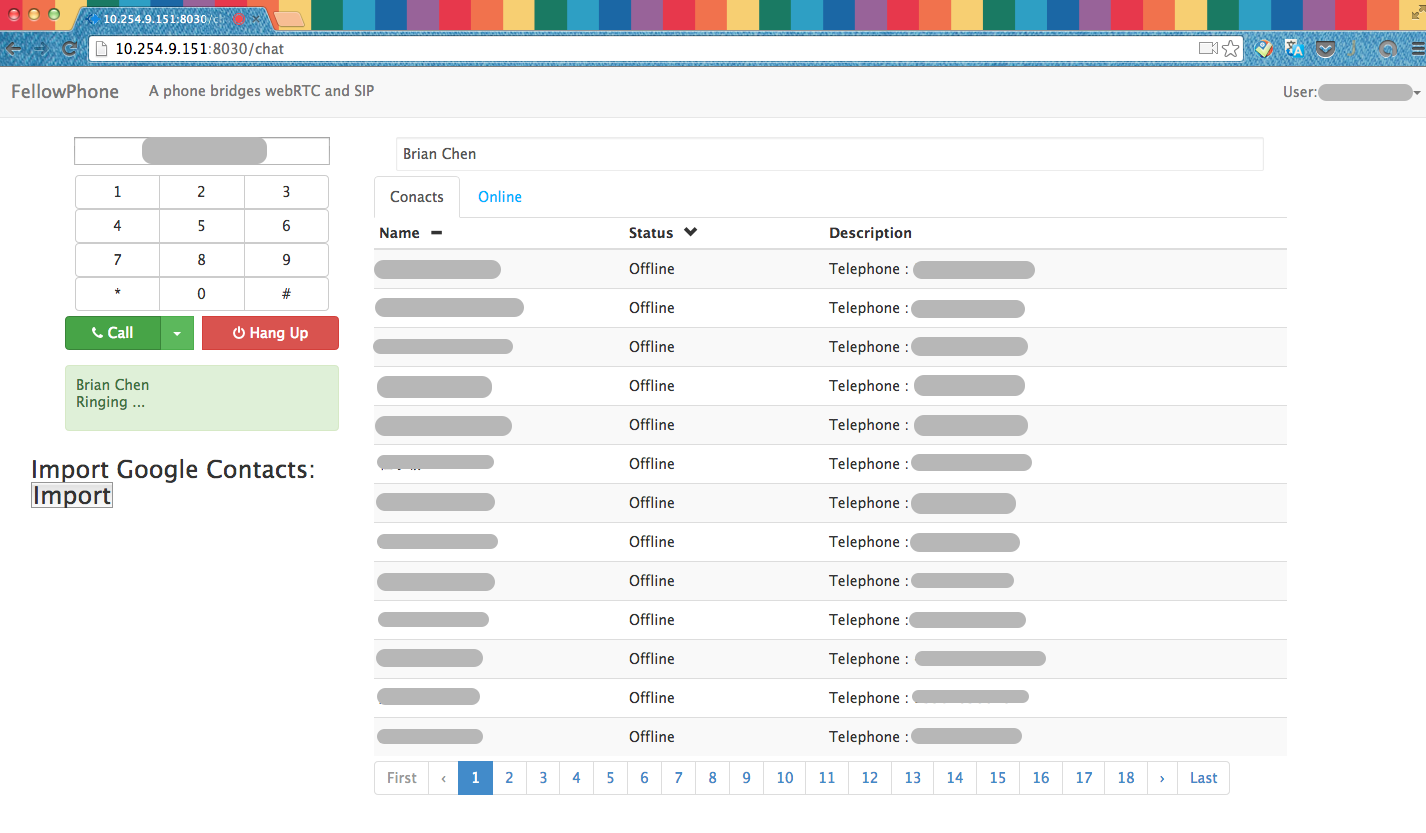
\includegraphics[width=0.90\textwidth,natwidth=610,natheight=642]{figs/webgui_call_outgoing.png}
  	\caption{Prototype Application Calling Outbound Mobile Number}
  	\label{fig:webgui_call_outgoing}
\end{figure}

\begin{table}
\caption{\label{tab:functions}: Prototype System Functions}
\centering
\begin{tabular}{| c | p{3cm} | p{5.5cm} |}
\hline
No & Function & Detail \\ \hline
\#1 & Single Call & Web browser client application can call outbound \gls{sip} client and receive outbound \gls{sip} client calling \\ \hline
\#2 & Multiple Users Video Conference & Multiple Web browser clients can have video conference \\ \hline
\#3 & Multiple Clients Conference & Multiple web browser client and single \gls{sip} client conference session \\ \hline
\#4 & Forward Call & When one of two web browser clients leaves the current three end points(2 \gls{webrtc} clients and 1 \gls{sip} client) conference, this \gls{sip} phone call will be forwarded to the only \gls{webrtc} client in the current conference session \\ \hline
\#5 & Instance Message & Instance Message chatting board in the current conference session \\ \hline
\#6 & Instance Message to \gls{sms} & \gls{sms} messages will be sent to \gls{sip} client phone which is in the current video conference session \\ \hline
\#7 & Files Sharing & Files can be shared in the current video conference session with the \gls{webrtc} client in the conference \\ \hline
\#8 & Google Contacts Import & User can import their Google Contacts to the application clients for synchronize contacts list \\ \hline
\#9 & Web Notification & All the necessary application notification will be display through the browser web notification message \\
\hline
\end{tabular} 
\end{table}

\par In the prototype system function Table \ref{tab:functions}, functions \#1 to \#4 is the basic telephony functions, they are implemented by \gls{webrtc} \gls{api}, application server and XMS media server. The detail about them will be covered in \gls{webrtc} \gls{api}s Implementation section, \gls{sip} Implementation section and XMS Media Server section since they are the real time communication function for \gls{webrtc} and \gls{sip} clients.

\par Function \#5 is implemented by Socket.IO framework which is discussed in previous chapter. The implementation detail will be covered in Socket.IO Implementation section.
Function \#6 is the advanced function along with the function \#5, it is implemented in \gls{msg} which will be discussed in \gls{sms} Messaging section in the later chapter.

\par Function \#7 is implemented by Delivery.js framework not the original \gls{webrtc} \textit{RTCDataChannel}, more detail will be discussed in Files Sharing section.

\par Function \#8 is another advanced feature provided by prototype application, it is implemented by Google Contacts \gls{api} which will be covered in AngularJs Framework Implementation section as the sample code section for AngularJs framework.

\par Function \#9 is to make the web application more user friendly and more like traditional telephone usage scenario. It will not be covered in this thesis since the user experience is not the top priority object for this thesis.

\section{WebRTC APIs Implementation}

\noindent \gls{webrtc} components are accessed with JavaScript \gls{api}s. Currently in development are the Network Stream \gls{api}, which represents an audio or video data stream, and the PeerConnection \gls{api}, which allows two or more users to communicate browser-to-browser. Also under development is a DataChannel \gls{api} which enables communication of other types of data for real-time gaming, text chat, file transfer, and so forth. Because the media server used in prototype system is not support for DataChannel yet, the DataChannel \gls{api} will not be covered in this section. \textit{RTCDataChannel} \gls{api} will be discussed in chapter \ref{chp:future_work}.

\begin{figure}
	\centering
    	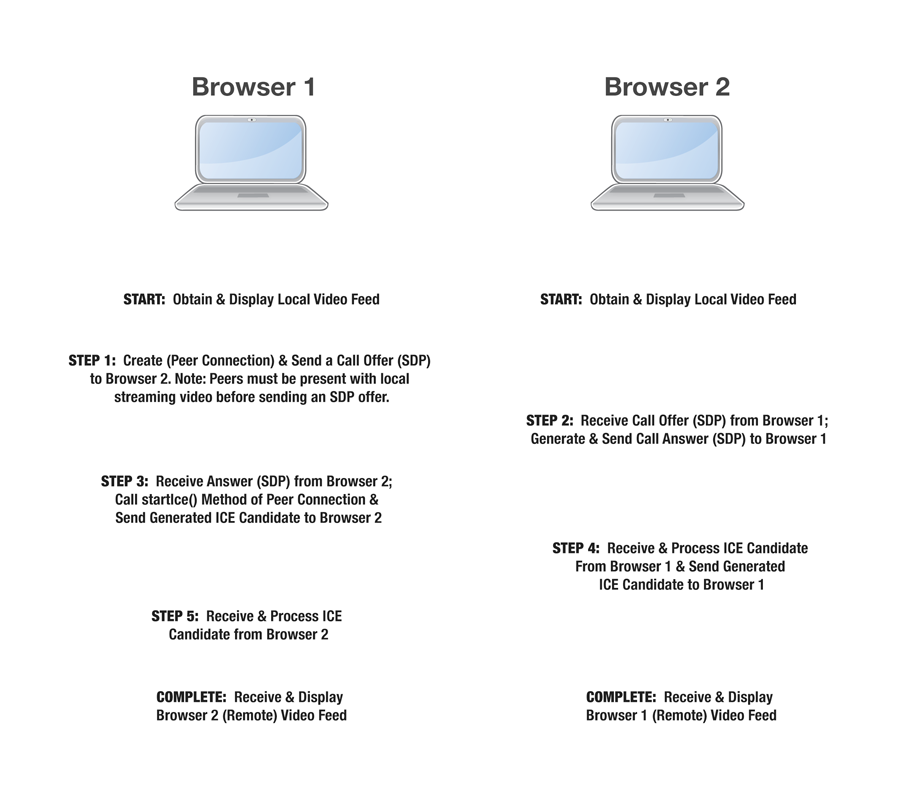
\includegraphics[height=0.50\textheight,natwidth=610,natheight=642]{figs/webrtc_diagram.png}
  	\caption{WebRTC two peer communication process\cite{mdn:p2pwebrtc}}
  	\label{fig:webrtc_diagram}
\end{figure}

\subsection{MediaStream API}

\par The MediaStream \gls{api} represents synchronized streams of media. For example, a stream taken from camera and microphone input has synchronized video and audio tracks. In order to obtain local media, the start step for both peers in Figure \ref{fig:webrtc_diagram}, the \gls{webrtc} \gls{api} provides \textit{navigator.getUserMedia()} function to get the video and audio stream from user. For privacy reasons, a web application’s request for access to a user’s microphone or camera will only be granted after the browser has obtained permission from the user. Each MediaStream has an input, which might be a MediaStream generated by \textit{navigator.getUserMedia()}, and an output, which might be passed to a video element or an \textit{RTCPeerConnection}.
\par The \textit{getUserMedia()} method takes three parameters:

\begin{itemize}[topsep=-1em,parsep=0em,itemsep=0em]
 \item A constraints object.
 \item A success callback which, if called, is passed a MediaStream.
 \item A failure callback which, if called, is passed an error object.
\end{itemize}

\par The Code Snippet \ref{code:get_user_media} shows that how the prototype application implements \textit{getUserMedia()} function, it is encapsulated in \textit{WebRTCService} (service is a reusable business logic independent of views in prototype application regarding to AngularJs framework\footnote{AngularJS is an open-source web application framework, maintained by Google and community, that assists with creating single-page applications, one-page web applications that only require HTML, CSS, and JavaScript on the client side.\cite{wiki:angularjs}}).For the constraints object in parameters, the prototype application set 'audio' and 'video' value to true because it is necessary for the real-time communication application to have video and audio stream both.

\begin{lstlisting}[caption={Get User Media Stream function},label={code:get_user_media}]
var media_constraints = {audio: true,video: true};

function _setMediaStream(){
	WebRTCService.getUserMedia(media_constraints,
  								_handleUserMedia,
  								_handleUserMediaError);
  	console.log('Getting user media with constraints', 
  				media_constraints);
}
\end{lstlisting}

\par \textit{getUserMedia()} function is currently available in Chrome, Opera and Firefox. Almost all of the \gls{webrtc} \gls{api}s are slightly different based on different browsers implementation. In the Code Snippet \ref{code:webrtc_service}, there are two blocks to make all the set up process for FireFox and to make the same set up process for Google Chrome. Because \gls{webrtc} is not standard Web \gls{api} yet, so the implementation on different browsers are different as well. For example, the \textit{RTCPeerConnection} \gls{api} in Firefox is \textit{mozRTCPeerConnection} but in Google Chrome it is \textit{webkitRTCPeerConnection}. In order to make the \gls{webrtc} application works on more browsers, the client side need to figure out which kind of browser is using on the machine then call the corresponding \gls{webrtc} \gls{api}s. Google provides a JavaScript shim called \textit{adapter.js}. It is maintained by Google, it abstracts away browser differences and spec changes. For Angularjs framework used by prototype application, then the \textit{WebRTCService} is implemented to be integrated with \textit{adapter.js} function to achieve the goal of compatibility.

\par However, the prototype application in this thesis will only focus on Google Chrome browser\footnote{Google Chrome is a freeware web browser developed by Google. It used the WebKit layout engine until version 27 and, with the exception of its iOS releases, from version 28 and beyond uses the WebKit fork Blink.\cite{wiki:google_chrome}} to simplify the development process because \gls{webrtc} lower level implementation on different browsers are different and hard to track the issues. Then most of the results in this thesis is based on the application performance of Google Chrome browser. The reason to choose Google Chrome browser rather than other browser because \gls{webrtc} is the technology rapidly pushed by Google and Google Chrome browser has the most market share in the world. As of March 2014, StatCounter estimates that Google Chrome has a 43\% worldwide usage share of web browsers, making it the most widely used web browser in the world.\cite{wiki:google_chrome} However, Google changes a lot to improve the performance of \gls{webrtc} on Google Chrome browser, then it makes the \gls{webrtc} \gls{api}s work differently on different version of Google Chrome browser. In the Code Snippet \ref{code:webrtc_service}, from line 19 to line line 29 is the sample case to distinguish the difference among different version of Google Chrome to handle the \textit{RTCPeerConnection} \gls{ice} server constraint implementation.

\begin{lstlisting}[caption={WebRTCService.js in application client},label={code:webrtc_service}]
angular.module('webrtcDemo.services').
	factory('WebRTCService',function () {
		
		...

		function _setRTCElement() {

			if(navigator.mozGetUserMedia){
				...
			}else if(navigator.webkitGetUserMedia){
				...

			  // Creates iceServer from the url for Chrome.
			  _createIceServer = function(url, username, password) {
			    ...
			    if (url_parts[0].indexOf('stun') === 0) {
			      ...
			    } else if (url_parts[0].indexOf('turn') === 0) {
			      if (_webrtcDetectedVersion < 28) {
			        // For pre-M28 chrome versions use old TURN format.
			        var url_turn_parts = url.split("turn:");
			        iceServer = { 'url': 'turn:' + username + '@' + url_turn_parts[1],
			                      'credential': password };
			      } else {
			        // For Chrome M28 & above use new TURN format.
			        iceServer = { 'url': url,
			                      'credential': password,
			                      'username': username };
			      }
			    }
			    return iceServer;
			  };

			  ...
			}else{
				console.log("Browser does not appear to be WebRTC-capable");
			}

		}

		return {
			...
		}
	});	
	
\end{lstlisting}

\par Since \gls{webrtc} \gls{api}s is not standard \gls{api} yet, the prototype application in this thesis will not pay too much work-load on compatibility for different browsers platform. More detail about this issue will be discussed in the Chapter \ref{chp:future_work}.

\subsection{RTCPeerConnection API}

\noindent The step 1 of Figure \ref{fig:webrtc_diagram} is that the caller peer set up a communication process, it simply creates \textit{RTCPeerConnection} then send a \gls{webrtc} offer(by calling \textit{createOffer()} function and sending WebSocket message with \gls{sdp}) with local \gls{sdp} to the other peer. In the prototype system, it will send \gls{webrtc} offer to the application server, then the application server will check if the receiver is a \gls{webrtc} client or \gls{sip} to send different type of offer message(It will be covered in later of this chapter).

\par To set up peer connection, the \textit{RTCPeerConnection} \gls{api} sets up a connection between two peers. In this context, “peers” means two communication endpoints on the World Wide Web. Instead of requiring communication through a server, the communication is direct between the two entities. In the specific case of \gls{webrtc}, a peer connection is a direct media connection between two web browsers. This is particularly relevant when a multi-way communication such as a conference call is set up among three or more browsers. Each pair of browsers will require a single peer connection to join them, allowing for audio and video media to flow directly between the two peers. 

\par To establish peer connection, it requires a new \textit{RTCPeerConnection} object. The only input to the \textit{RTCPeerConnection} constructor method is a configuration object containing the information that \gls{ice}, will use to “punch holes” through intervening \gls{nat} devices and firewalls. The Code Snippet \ref{code:create_peer_connection} shows the create \textit{RTCPeerConnection} object and set three listener (\textit{onicecandidate},\textit{onaddstream},\textit{onremovestream}) to trigger the handlers to deal with the \gls{ice} candidate event and remote stream add/remove events.

\par The \textit{RTCPeerConnection} \gls{api} has two arguments to set, one is configuration object for peer connection and the other is constraint object (set transparent protocol and encryption) for peer connection, these value are shown in Code Snippet \ref{code:create_peer_connection} line 1 to line 10. In the showing case, the prototype is using \gls{stun} servers for different browser aspect, and set the \gls{rtc} channel encryption protocol to \gls{dtls}\footnote{In information technology, the Datagram Transport Layer Security (DTLS) protocol provides communications privacy for datagram protocols. DTLS allows datagram-based applications to communicate in a way that is designed to prevent eavesdropping, tampering, or message forgery.\cite{wiki:dtls}} and enable the \gls{rtc} DataChannel.

\par Because in Firefox, \gls{webrtc} media transparent channel is only based on \gls{dtls} protocol, and in latest version Google Chrome, \gls{dtls} is supported, then in the prototype application, it will use \gls{dtls} protocol to exchange the media stream.

\par There are two \gls{api}s to handle the \textit{RTCIceCandidate} object which contains \gls{ice} information data. One is \textit{onicecandidate} listener to trigger the function to handle the new \textit{RTCIceCandidate} data object. The other one is \textit{addIceCandidate} function, which is shown in the Code Snippet \ref{code:add_remote_ice}, to add the new \textit{RTCIceCandidate} data object to the remote/local peer connection session description field. As Code Snippet \ref{code:add_remote_ice} shown, the \textit{RTCIceCandidate} object has three attributes, \textit{sdpMLineIndex} is the media line index in the \gls{sdp}, \textit{sdpMid} is the media id which differ it is video or audio in the \gls{sdp} and \textit{candidate} is the \gls{ip} address and other detail of this media source.

\begin{lstlisting}[caption={Create Peer Connection function},label={code:create_peer_connection}]
pc_config = WebRTCService.webrtcDetectedBrowser() === 'firefox' ?
  			{'iceServers':[{'urls':'stun:stun.services.mozilla.com'}]} :
  			{'iceServers':[{'urls': 'stun:stun.l.google.com:19302'}]};

pc_constraints = {
			  'optional': [
			    {'DtlsSrtpKeyAgreement': true},
			    {'RtpDataChannels': true}
			  ]
			};
			
function _createPeerConnection(){

	try {
		pc = WebRTCService.peerConnection(pc_config, pc_constraints);
		pc.onicecandidate = _handleIceCandidate;
		console.log('Created RTCPeerConnnection with:\n' +
		      '  config: \'' + JSON.stringify(pc_config) + '\';\n' +
		      '  constraints: \'' + JSON.stringify(pc_constraints) + '\'.');
	} catch (e) {
		console.log('Failed to create PeerConnection, exception: ' + e.message);
		alert('Cannot create RTCPeerConnection object.');
		return;
	}
	pc.onaddstream = _handleRemoteStreamAdded;
	pc.onremovestream = _handleRemoteStreamRemoved;

}
\end{lstlisting}

\begin{lstlisting}[caption={Add Remote IceCandidate function},label={code:add_remote_ice}]
var candidate = WebRTCService.RTCIceCandidate({
					    	sdpMLineIndex:data.content.label,
					    	sdpMid:data.content.id,
					    candidate:data.content.candidate
				});
pc.addIceCandidate(candidate);

\end{lstlisting}

\par There are difference between Firefox and Google Chrome to handle the \textit{RTCIceCandidate} content in the \gls{sdp} while sending the offer to the other peer. In Firefox, it waits for all the \textit{RTCIceCandidate} data is fetched from \gls{stun}/\gls{turn} server then send it with \gls{webrtc} offer message. However, in Google Chrome, it sends the \gls{webrtc} offer message first, then update the local \gls{sdp} with new coming \textit{RTCIceCandidate} data one by one. Then in the prototype system, it needs to handle these differences by listening the \textit{endIceCandidate} event on application. After client fetches all the \textit{RTCIceCandidate} data, it sends an \textit{endIceCandidate} message to the application server to send the complete \gls{webrtc} offer message to the other peer.

\par In the step 2 of Figure \ref{fig:webrtc_diagram}, after the caller \textit{RTCPeerConnection} run \textit{createOffer()} function to send offer to callee through signaling channel, the callee need run \textit{createAnswer()} function to ask the \gls{stun}/\gls{turn} server to find the path for each other peer and create the answer with \gls{sdp} content. \gls{sdp} is intended for describing multimedia communication sessions for the purposes of session announcement, session invitation, and parameter negotiation. \gls{sdp} does not deliver media itself but is used for negotiation between end points of media type, format, and all associated properties.\cite{wiki:sdp} Before \textit{RTCPeerConnection} use \textit{createOffer()} function to send a \gls{webrtc} offer to the callee, it is required to be present with local streaming video, like Figure \ref{fig:webrtc_diagram} mentioned.

\par \gls{webrtc} clients need to ascertain and exchange local and remote audio and video media information, such as resolution and codec capabilities. Signaling to exchange media configuration information proceeds by exchanging an offer and an answer using the \gls{sdp}. The \textit{createOffer()} function and \textit{createAnswer()} function both have callback function to handle the \gls{sdp} either to call \textit{setLocalDescription()} by caller or call \textit{setRemoteDescription()} by callee when callee gets the caller's \gls{sdp} from \gls{webrtc} offer. The Code Snippet\ref{log:webrtc_answer_sdp} shown is the \gls{webrtc} answer \gls{sdp} from the callee when the callee end-point decide to accept this conversion session.

\par The sample \gls{sdp} from the prototype application is shown in Code Snippet \ref{log:webrtc_answer_sdp}. Line 2 in Code Snippet \ref{log:webrtc_answer_sdp} is the field 'o', it describes originator, session identifier, username, id, version number and network address. It usually means that where this package comes from. Line 7 and line 17 are field 'm', it describes media name and transport address. And line 11,12 and line 27,28 are the relevant lines for audio and video media field, they describes media filed 'candidate' attributes, in the sample case of Code Snippet \ref{log:webrtc_answer_sdp}, they are the \gls{ice} candidate from the \gls{stun}/\gls{turn} server. These are important fields regarding to the prototype system because they are used in XMS server and application server of the prototype system to exchange the media stream.

\begin{lstlisting}[caption={Sample \gls{webrtc} Answer \gls{sdp}},label={log:webrtc_answer_sdp}]
sdp: v=0
o=xmserver 1399363527 1399363528 IN IP4 10.254.9.135
s=xmserver
c=IN IP4 10.254.9.135
t=0 0
a=ice-lite
m=audio 49152 RTP/SAVPF 0 126
a=rtpmap:0 PCMU/8000
a=sendrecv
a=rtcp:49153
a=candidate:1 1 UDP 2130706431 10.254.9.135 49152 typ host
a=candidate:1 2 UDP 2130706430 10.254.9.135 49153 typ host
...
a=acfg:1 t=1
a=rtpmap:126 telephone-event/8000
a=fmtp:126 0-15
m=video 57344 RTP/SAVPF 100
b=AS:1000
a=rtpmap:100 VP8/90000
a=fmtp:100 max-fr=30; max-fs=1200
a=sendrecv
a=rtcp:57345
a=rtcp-fb:100 ccm fir
a=rtcp-fb:100 nack
a=rtcp-fb:100 nack pli
a=rtcp-fb:100 goog-remb
a=candidate:2 1 UDP 2130706431 10.254.9.135 57344 typ host
a=candidate:2 2 UDP 2130706430 10.254.9.135 57345 typ host
...
\end{lstlisting}

\par In the step 3 of Figure \ref{fig:webrtc_diagram}, the caller will receive the answer from callee and process it by adding the remote \gls{sdp} to \textit{RTCPeerConnection}, like the Code Snippet \ref{code:add_remote_ice}. By the meantime, the step 4 of Figure \ref{fig:webrtc_diagram}, the callee will receive the \gls{sdp} from caller with the \gls{ice} candidate information data, and process it the same way as caller does, add some to \textit{RTCPeerConnection} object by \textit{addIceCandidate()} function. In the prototype system, these exchange \textit{RTCIceCandidate} process is relayed by application server to the different end points.

\par Once the \textit{RTCPeerConnection} is established, the client need configure where the media or data to store and display if it is necessary. In the prototype application of this thesis, media stream will be displayed in a \gls{html5} tag called \textit{<video>}. It will only be shown when there is media stream in \textit{<video>} tag source.

\section{AngularJs Framework Implementation}

\noindent As it described about AngularJs in Chapter \ref{chp:pre_study}, there are three layer components in the framework, view, controller and service. The files structure is shown in Appendix \ref{code:angularjs_structure}. Application has two main web pages, \textit{login} page and \textit{phone} page. There are \textit{chatboard},\textit{contacts list}, \textit{contacts table}, \textit{dialpanel} and \textit{notification} user interface component blocks in \textit{phone} page. For each part of the application blocks, it has controller script and service script. Controller and service scripts are working with the \gls{html} view scripts. In this section, there will be one sample component block of the prototype application client explained in order to understand how the AngularJs is used in prototype application.

\par The \textit{app.js} script shown in Code Snippet \ref{code:app_js} is the bootstrap script for AngularJs framework. It initializes the application module of AngularJs framework and declare the dependencies which will be used in the application.

\par The contact table component in \textit{phone} page of the application is structured in four scripts, \textit{contactTable.jade} script in Code Snippet \ref{code:contact_table}, \textit{ContactTableDirective.js} script in Code Snippet \ref{code:contact_table_dir}, \textit{ContactsCtrl.js} script in Code Snippet \ref{code:contact_ctrl} and \textit{GoogleAPIService.js} script in Code Snippet \ref{code:google_api}. It provides the application contacts information in advanced functioning table and search function in text input filed.

\subsection{app.js Script (AngularJs Bootstrap)}

\par The \textit{app.js} script shown in Code Snippet \ref{code:app_js}, it declares the application level module which depends on different filters, modules and services. The modules \textit{webrtcDemo.services}, \textit{webrtcDemo.controllers}, \textit{webrtcDemo.directives} and \textit{webrtcDemo.filters} are the customized modules implemented for prototype application. The rest of the modules included as dependencies are third party AngularJs modules used in the prototype application. AngularJs developer community is quite active community, there are many useful open sourced projects or modules can be just included for using in the prototype application.

\par In Code Snippet \ref{code:app_js}, from line 8 to line 20 is implemented to set the application routing map. There are two main pages, one is \textit{login} page with "/login" \gls{url} and the other one is \textit{phone} page with "/chat" \gls{url}. The Angular controllers which are bind with these page view are also declared in \textit{\$routeProvider} service. And the default \gls{url} is set to "/login" to make sure if user has not logged in the system, he need to input the user credential to enter the service. 

\label{app:app_js}
\begin{lstlisting}[caption={app.js in application client},label={code:app_js}]
angular.module('webrtcDemo', [
    ...
  'webrtcDemo.services',
  'webrtcDemo.controllers',
  'webrtcDemo.directives',
  'webrtcDemo.filters'
]).
config(function ($routeProvider, $locationProvider, $httpProvider) {
  $routeProvider.
    when('/chat', {
      templateUrl: 'partials/phoneView',
      controller: 'PhoneViewCtrl'
    }).
    when('/login',{
      templateUrl: 'partials/login',
      controller: 'LoginViewCtrl'
    }).
    otherwise({
      redirectTo: '/login'
    });

  ...
  });

\end{lstlisting}

\subsection{contactTable.jade Script (View)}

\par The \textit{contactTable.jade} script is the view component of the AngularJs. It is a Jade\footnote{Jade is a high performance template engine heavily influenced by Haml and implemented with JavaScript for node.\cite{github:jade}} script file. The template engine used on Node.js in prototype application is Jade which provides more clear way to program \gls{html} node template scripts than normal \gls{ejs} template engine. In Code Snippet \ref{code:contact_table}, Jade has the same node name as \gls{ejs}. And there are some Angular directives in the template from Code Snippet \ref{code:contact_table}. For example, at line 2 in Code Snippet \ref{code:contact_table}, the \textit{angucomplete-alt} directive is a third party Angular directive to provide auto-completion features in \gls{html} \textit{<input>} text tag. The different attributes in the \textit{angucomplete-alt} node is to set some configuration to this directive, like the attribute field \textit{local-data} is the array data to search for content as auto-complete reference.

\par Moreover, AngularJs itself provides native Angular directive as well. For instance, at line 11 in Code Snippet \ref{code:contact_table}, the attribute \textit{ng-class} is a native Angular directive attribute, it provides the \gls{css}\footnote{Cascading Style Sheets (CSS) is a style sheet language used for describing the look and formatting of a document written in a markup language.\cite{wiki:css}} changes to some specific \gls{css} class name according to some certain value matches in AngularJs expression. At line 11, the \textit{<tr>} tag's \gls{css} attributes will be success \gls{css} class only if the boolean value of \textit{item.online} is \textit{true}.

\par AngularJs provides two-way data module binding in the template and controller. Line 17 in the Code Snippet \ref{code:contact_table}, \textit{\{\{item.number\}\}} is the Angular template to display the \textit{number} property value of \textit{item} object in the \gls{html} template. And line 14 is the example of Angular template integrated with Angular filter, the third-party filter \textit{iif} here is the filter to check the \textit{\{\{item.online\}\}} value if it is \textit{true} or \textit{false}. If it is \textit{true} then it will show \textit{Online} string text in the \gls{html} template otherwise it will show \textit{Offline} string text. The syntax here is quite similar to any other programming language.

\begin{lstlisting}[caption={contactTable.jade in application client},label={code:contact_table}]
div(id = "contactTable")
	angucomplete-alt(id="contactSearch",
		...
		local-data="contactsHolder.contacts",
		...)
	tabset
		tab(heading = "Conacts")
			table(id = "contacts", at-table, at-paginated, at-list="contactsHolder.contacts | orderBy:online", at-config="config",class="table table-hover table-striped table-condensed" )
				thead
				tbody
					tr(ng-class = "{success: item.online}", ng-init = "item.hvor = false", ng-mouseenter = "contactHvor(item)", ng-mouseleave = "contactHvor(item)")
						...
							p(ng-hide = "item.hvor").
								{{item.online | iif : "Online" : "Offline" }}
                        ...
							p
								| Telephone : {{item.number}}
			...
\end{lstlisting}

\subsection{ContactTableDirective.js Script (Customized Directive)}

\par After creating the view of contact table component, it is necessary to bind controller to the view and declare the component a tag name used in the \gls{html} template. It is called \textit{Directive} in AngularJs, and the \textit{ContactTableDirective.js} script is shown in Code Snippet \ref{code:contact_table_dir}. From line 1 to line 12 is the directive declaration, it sets the \textit{templateUrl} to 'partials/contactTable' which is the view component file path and binds the controller which named as \textit{ContactsCtrl} to the view component. The \textit{restrict} filed in the directive is to set the template type for \textit{ContactTableDirective}, in the Code Snippet \ref{code:contact_table_dir} line 5, it means this directive is a \gls{html} element template, it can be used as normal \gls{html} element by using name 'contact-table'. By using AngularJs directive, it makes the \gls{html} view template more modularized and makes the same view component could be reused in different place in the web application.

\par From line 14 to line 19 is the Angular filter declaration, it is a filter named as  \textit{iif}, the only function it does is to check the \textit{input} value and return \textit{trueValue} if \textit{input} is \textit{true} otherwise return \textit{falseValue}. The usage is described in previous section at line 14 of the Code Snippet \ref{code:contact_table}.

\begin{lstlisting}[caption={ContactTableDirective.js in application client},label={code:contact_table_dir}]
angular.module('webrtcDemo.directives').
	directive('contactTable',function () {

		return{
			restrict: 'E',
			replace: true,
			scope: true,
			templateUrl: 'partials/contactTable',
			controller: 'ContactsCtrl'
		};

	});

angular.module('webrtcDemo.filters').
	filter('iif', function () {
   return function(input, trueValue, falseValue) {
        return input ? trueValue : falseValue;
  };
});
\end{lstlisting}

\subsection{ContactsCtrl.js Script (Controller)}

\par The controller in AngularJs is to control the user interface logic and bridge the data business logic from the services with the user interface views. The example controller in Code Snippet \ref{code:contact_ctrl} controls the contactTable view directive and get data functions from GoogleAPIService. At the line 2 of Code Snippet \ref{code:contact_ctrl}, in the controller construction function, there are several services arguments. They are the services this controller will use in the application, one of them is \textit{GoogleAPIService} which is related to the contacts information data. The contactTable view directive need contacts information data to show in the \gls{html} template. And \textit{storage} is another service provides \textit{localstorage} function in \gls{html5} application. This service is used to store the contacts information data locally to make user no need to import his Google contacts information all the time. This function is implemented at line 22 of the Code Snippet \ref{code:contact_ctrl} by calling \textit{storage.set()} function to store the contacts data in the \gls{w3c} web storage.

\par At line 5 of the Code Snippet \ref{code:contact_ctrl}, it is the function \textit{\$scope.importContacts}, the reason this function is under \textit{\$scope} object is because this function is directly triggered by one \gls{ui} button. In this function, there are two Javascript promise functions from the \textit{GoogleAPIService} used. One is \textit{GoogleAPIService.oAuth()} function which is to ask user to get Google \gls{api} permission to query the Google Contacts \gls{api}. The other one is  to query the contacts information data by Google Contacts \gls{api} after get the Google \gls{api} permission.

\par \textit{Promise} object is the new concept in the AngularJs, and it will be standardized in new ECMAScript\footnote{ECMAScript is the scripting language standardized by Ecma International in the ECMA-262 specification and ISO/IEC 16262. The language is widely used for client-side scripting on the web, in the form of several well-known implementations such as JavaScript, JScript and ActionScript.\cite{wiki:ecmascript}} 6. The core idea behind promises is that a promise represents the result of an asynchronous operation. A promise object is in one of three different states:\cite{website:promise}
\begin{itemize}[topsep=-1em,parsep=0em,itemsep=0em]
 \item \textbf{Pending} - The initial state of a promise.
 \item \textbf{Fulfilled} - The state of a promise representing a successful operation.
 \item \textbf{Rejected} - The state of a promise representing a failed operation.
\end{itemize}

\par It is a great concept and important feature in the AngularJs. Since everything in Javascript is asynchronous operation, then promise function is used to deal with the function calling after previous asynchronous operation success. The implementation of these two promise functions will be covered in the next section of AngularJS service.

\par From line 9 to line 15 is the process to strip the useful information from the response data to get the correct contact information into \textit{contact} object, then push them one by one into a \textit{contact} object array in order to use the contacts list in contact table view component.

\begin{lstlisting}[caption={ContactsCtrl.js in application client},label={code:contact_ctrl}]
angular.module('webrtcDemo.controllers').
	controller('ContactsCtrl',function ($scope,$location,WebSocketService,GoogleAPIService,storage,$filter) {
		...
		
		$scope.importContacts = function(){
			$scope.contactsHolder.contacts = [];
			GoogleAPIService.oAuth().then(function(token){
				GoogleAPIService.queryContacts(token).then(function(data){
					angular.forEach(data.feed.entry,function(person, key){
						if(person['gd$phoneNumber']){
							var contact = {
								name: person.title['$t'],
								number: person['gd$phoneNumber'][0]['$t'],
								online: false
							}

							...

						}
					});

					storage.set('contactList-' + username,$scope.contactsHolder.contacts);

				});
			});
		}

	});
\end{lstlisting}


\subsection{GoogleAPIService.js Script (Service)}

\par AngularJs service provides most of the business logic of the application. Like the sample code shown in Code Snippet \ref{code:google_api}, it provides interfaces of Google \gls{api} to the controller. There are two interfaces in the \textit{GoogleAPIService.js} script. One is Google authorization login to get the user permission, the other one is fetching Google contacts information from the Google Contacts \gls{api}.

\par From line 4 to line 20 in Code Snippet \ref{code:google_api}, it is the promise function, \textit{\_authLogin()}, to get Google authorization token in order to call any Google \gls{api}s later. It uses \textit{\$q} service from AngularJs to provide \textit{deferred} \gls{api} and \textit{prmoise} \gls{api}. The purpose of the deferred object is to expose the associated \textit{prmoise} instance as well as \gls{api}s that can be used for signaling the successful or unsuccessful completion, as well as the status of the task.The purpose of the \textit{prmoise} object is to allow for interested parties to get access to the result of the deferred task when it completes.\cite{angular:q} At line 5 and line 23 is the code to create a new instance of \textit{deferred} and a new \textit{prmoise} instance. From line 7 to 10, it is the configuration object for Google \gls{api} authorization. The \textit{gapi} object is loaded from the Google \gls{api} Javascript client script included in \textit{index.jade} shown in Code Snippet \ref{code:include_googleapi}.

\begin{lstlisting}[caption={Include Google API Javascript file in Index.iade},label={code:include_googleapi}]
script(src='https://apis.google.com/js/client.js' type='text/javascript')
\end{lstlisting}

\par Since application only needs to get permission form user Google Contacts, then the scope is set to \url{https://www.google.com/m8/feeds} and the client\_id is got from the Google App Engine (\url{https://console.developers.google.com}). Developer needs to create his own Google App project then set the \gls{api}s which the project will ask user permission for and the credentials used for client or web service. In the prototype system, it is the web application client to use the Google Contacts \gls{api} then there is a client \gls{oauth} 2.0\footnote{OAuth is an open standard for authorization. OAuth provides client applications a 'secure delegated access' to server resources on behalf of a resource owner.OAuth 2.0 is the next evolution of the OAuth protocol and is not backwards compatible with OAuth 1.0. OAuth 2.0 focuses on client developer simplicity while providing specific authorization flows for web applications, desktop applications, mobile phones, and living room devices.\cite{wiki:oauth}} credential created on Google App project.

\par Then the \textit{gapi} object call \textit{auth.authorize()} function with the configuration object to get authorization token. At line 15, when the asynchronous process is finished, \textit{deferred} object will call \textit{resolve} function to send the token object back to the \textit{promise.then} function at line 7 in Code Snippet \ref{code:contact_ctrl} which is mentioned at previous section.

\par From line 22 to line 34 in Code Snippet \ref{code:google_api} is another promise function, \textit{\_fetchContacts()} , to fetch the Google contacts information data after getting user permission to use their Google service data. This function makes a \gls{http} request in \gls{jsonp} to fetch all the contacts information from Google Contacts \gls{api}. \gls{jsonp} is a communication technique used in JavaScript programs running in web browsers to request data from a server in a different domain, something prohibited by typical web browsers because of the same-origin policy. \gls{jsonp} takes advantage of the fact that browsers do not enforce the same-origin policy on \textit{<script>} tags\cite{wiki:jsonp}. The reason application uses \gls{jsonp} in \gls{http} request is that web application is host in one origin domain and Google \gls{api} server is in another origin domain, it is cross domain request when prototype application requests for data from Google \gls{api} server. And Google \gls{api} server does not support cross domain request for security, but with \gls{jsonp} it is allowed to have cross origin domain resources sharing.

\par The \textit{\_fetchContacts()} function uses the same mechanism as \textit{\_authLogin()} function described above to make promise function, it returns contacts information data from Google Contacts \gls{api} as the promise function resolving data, shown at line27 in Code Snippet \ref{code:google_api}.

\begin{lstlisting}[caption={GoogleAPIService.js in application client},label={code:google_api}]
angular.module('webrtcDemo.services').
	factory('GoogleAPIService', function ($q,$http,storage) {

		function _authLogin(){
			var deferred = $q.defer();

			var config = {
		      'client_id': 'xxxxxxxxxxxxxxx.apps.googleusercontent.com',
		      'scope': 'https://www.google.com/m8/feeds'
		    };
	    gapi.auth.authorize(config, function() {

	      console.log('login complete');
	      console.log(gapi.auth.getToken());
	      deferred.resolve(gapi.auth.getToken());

	    });

	    return deferred.promise;
		}

		function _fetchContacts(authToken){
			...
			
			$http.jsonp(url).
	    success(function(data, status, headers, config) {
	      deferred.resolve(data);
	    }).
	    error(function(data, status, headers, config) {
	      deferred.reject('GoogleAPIService:queryContacts:Failed');
	    });

			return deferred.promise;
		}

		...
	});
\end{lstlisting}

\section{Socket.IO Implementation}

\noindent In the prototype system, web application client and application server communicate with each other over WebSocket shown in Figure \ref{fig:system_network}. There are two main intentions to have the signaling channel over WebSocket. One is for signaling of \gls{webrtc} \gls{ice} candidate exchange and the other one is to exchange the communication data (text message, files). Unlike \gls{http}, WebSocket provides full-duplex communication. Additionally, Websocket enables streams of messages on top of \gls{tcp}. \gls{tcp} alone deals with streams of bytes with no inherent concept of a message. Before WebSocket, port 80 full-duplex communication was attainable using Comet\footnote{Comet is a web application model in which a long-held HTTP request allows a web server to push data to a browser, without the browser explicitly requesting it.Comet is an umbrella term, encompassing multiple techniques for achieving this interaction. All these methods rely on features included by default in browsers, such as JavaScript, rather than on non-default plugins. The Comet approach differs from the original model of the web, in which a browser requests a complete web page at a time.\cite{wiki:comet}} channels; however, Comet implementation is nontrivial, and due to the \gls{tcp} handshake and \gls{http} header overhead, it is inefficient for small messages. WebSocket protocol aims to solve these problems without compromising security assumptions of the web.\cite{wiki:websocket}

\begin{table}
\caption{\label{tab:websocket}: Socket.IO Listening Channels in Code Snippet \ref{code:server_socket}}
\centering
\begin{tabular}{| c | p{3cm} | p{5.5cm} |}
\hline
 WebSocket Channel & Message Data Type & System Function \\ \hline
 \multicolumn{1}{ |c }{\multirow{3}{*}{\gls{sip}} } & \multicolumn{1}{ | p{3cm} | }{register} &  Web application login page \gls{sip} registeration message to \gls{sip} server\\ \cline{2-3}
 \multicolumn{1}{ |c  }{} & \multicolumn{1}{ | p{3cm} | }{invite} & Web application client invites \gls{sip} client message \\ \cline{2-3}
 \multicolumn{1}{ |c  }{} & \multicolumn{1}{ | p{3cm} | }{answerInvite} & Web application client gets INVITE \gls{sip} message from \gls{sip} client and answers it \\ \cline{1-3}
 \multicolumn{1}{ |c }{\multirow{5}{*}{\gls{webrtc}} } & \multicolumn{1}{ | p{3cm} | }{register} &  Web application client finishes login with \gls{sip} credential and gets user permission to use \textit{getUserMedia()} function and registers client itself on application server for WebSocket usage \\ \cline{2-3}
 \multicolumn{1}{ |c  }{} & \multicolumn{1}{ | p{3cm} | }{offer} & Web application client sends offer message to appliction server to create call resource on XMS media server \\ \cline{2-3}
 \multicolumn{1}{ |c  }{} & \multicolumn{1}{ | p{3cm} | }{answerInvite} & Web application client gets INVITE message from \gls{webrtc} client and answers it \\ \cline{2-3}
 \multicolumn{1}{ |c  }{} & \multicolumn{1}{ | p{3cm} | }{endCandidate} & Web application client finishes getting \gls{ice} candidate from \gls{stun}/\gls{turn} server then application sends \gls{http} request to XMS media server with final \gls{sdp} \\ \cline{2-3}
 \multicolumn{1}{ |c  }{} & \multicolumn{1}{ | p{3cm} | }{hangup} & Web application client sends hangup messge to hangup itself from the current conference \\ \cline{1-3}
 \multicolumn{1}{ |c }{\multirow{2}{*}{message} } & \multicolumn{1}{ | p{3cm} | }{\gls{im}} &  Web application sends instance message to application server in order to broadcast to all the rest clients in current conference\\ \cline{2-3}
 \multicolumn{1}{ |c  }{} & \multicolumn{1}{ | p{3cm} | }{\gls{sms}} & Web application client sends \gls{sms} to \gls{sip} client \\ \cline{1-3}
 disconnect & * &  Web application client disconnects from the application server\\ \hline
\end{tabular} 
\end{table}

\subsection{Server Side Implementation}

\par The Code Snippet \ref{code:server_socket}, it is implementation of Socket.IO on the application server. From line 1 to line 6, it is the initialization process of the Socket.IO on Node.js. At line 4, it means that when the client binds with the application server through WebSocket, the listener start in handler function \textit{\_handlerSocket()}. The WebSocket channels and usages are shown in Table \ref{tab:websocket}.

\par At line 11 in Code Snippet \ref{code:server_socket}, \textit{socket} object is created by the Socket.IO framework whenever one client connects with the server through WebSocket. The \textit{listener} function is implemented in the same pattern in \textit{socket.on()}. There are two arguments taken by this function. The first one is the channel name, at line 11, it is \textit{sip}, and second argument is callback function when this channel got any socket message. This callback function also takes one argument which is the message data sent by the client.

\par At line 16 in Code Snippet \ref{code:server_socket}, it is the implementation for server to send socket message back to the client through WebSocket in Socket.IO framework. \textit{socket.emit()}, this function takes two arguments, the first one is the WebSocket channel name and second one is the socket message data object. All the socket message data is formatted in \gls{json} because it is easier for both client and server side to resolve these message data.

\subsection{Client Side Implementation}

\par Since Socket.IO library is a library to make the communication channel between server and client, besides server side implementation, there is client side implementation which is correspond to the server side implementation.

\par The client side Socket.IO implementation is quite similar as the server side implementation mentioned above. The socket message event listener is implemented as the same pattern, like line 3 in Code Snippet \ref{code:client_socket}. Moreover, at line 15, \textit{socket.emit()} function is used for client to send socket message through WebSocket to server in Socket.IO framework. In this way, the client has same WebSocket channels listed in Table \ref{tab:websocket} and sends the related data type to the server to request server to run some corresponding process.

\begin{lstlisting}[caption={\_setSocketListener() Function in PhoneViewCtrl.js on Application Client},label={code:client_socket}]
function _setSocketListener(socket){

			socket.on('log', function (array){
			  console.log.apply(console, array);
			});

			socket.on('webrtc', function (data){
			  
			  switch(data.type){
			  	...
			  	case 'answer':
			  		if(isStarted){
			  			...
			  			if(!data.self){
			  				socket.emit('sip',{
						    	type: 'invite',
						    	username: $scope.user.name,
						    	content: {
						    		to: $scope.outPhone.number
						    	}
						    });
			  			}else{
			  				...
			  			}
			  		}
			  		break;
			  	...
			  }
			});

			...
		}

\end{lstlisting}


\section{SIP Implementation on Application Server}

\noindent There are not many \gls{sip} stack module made on \gls{npm}\footnote{npm is the official package manager for Node.js. As of Node.js version 0.6.3, npm is bundled and installed automatically with the environment. npm runs through the command line and manages dependencies for an application. It also allows users to install Node.js applications that are available on the npm registry.\cite{wiki:npm}}. After a lot of research, this prototype system will use a simple \gls{sip} module(sip.js ,\url{https://www.npmjs.org/package/sip}) on Node.js. It implements tranaction and transport layers as described in RFC3261(SIP: Session Initiation Protocol, \url{http://www.ietf.org/rfc/rfc3261.txt}). This library is still maintained by its author although the developer of this library is not so active during this thesis research period. But this library is the most appropriate library for Node.js.

\par The examples of sip.js library usage mostly are to be implemented as a \gls{sip} registration server or proxy server. Then the most of the interfaces provided by sip.js library are design to redirect all the \gls{sip} message and \gls{sip} register request. Although sip.js library provides \gls{sip} stack for Node.js and lower layer transportation on \gls{sip} protocol interface, it is not designed for manually generating different \gls{sip} message request to \gls{sip} server. Most of the \gls{sip} implementation of prototype application server have to be implemented to handle with all different types of \gls{sip} message generation cases by its own which is shown in Code Snippet \ref{code:sipjs}. These implementation is made based on the reference of RFC3261 and Wireshark\footnote{Wireshark is a free and open-source packet analyzer. It is used for network troubleshooting, analysis, software and communications protocol development, and education. Originally named Ethereal, in May 2006 the project was renamed Wireshark due to trademark issues.\cite{wiki:wireshark}} trace log of the \gls{sip} soft-phone application\footnote{A softphone is a software program for making telephone calls over the Internet using a general purpose computer, rather than using dedicated hardware.\cite{wiki:softphone}} (like Zoiper).

\subsection{SIP Request Message Implementation}

\par As mentioned in Chapter \ref{chp:intro}, there will be \textit{REGISTER},\textit{INVITE},\textit{ACK},\textit{CANCEL} and \textit{BYE} \gls{sip} message request implemented in application server to provide normal \gls{webrtc} browser client the \gls{sip} communication ability. Fortunately, the sip.js library provides mostly used \gls{sip} response, it is no need to modified these response when application server relaies the \gls{sip} response back to client.

\par From line 3 to line 20 of Code Snippet \ref{code:sipjs} , it is the code block for generating \textit{REGISTER} \gls{sip} message request. It is implemented regarding to RFC3261. The important part of this block implementation is the header of \textit{REGISTER} \gls{sip} message. There are \textit{call-id},\textit{cseq},\textit{from},\textit{to},\textit{contact} fields need to be set in the header. Field \textit{call-id} contains a globally unique identifier for this call, generated by the combination of a random string and the client's host name or \gls{ip} address. The combination of the \textit{to} tag, \textit{from} tag, and \textit{call-id} completely defines a peer-to-peer \gls{sip} relationship between two end points and is referred to as a dialog. Field \textit{cseq} or Command Sequence contains an integer and a method name. The \textit{cseq} number is incremented for each new request within a dialog and is a traditional sequence number. For the prototype application server, the \textit{cseq} number is increased (shown at line 69 of Code Snippet \ref{code:sipjs} ) when the \gls{sip} \textit{REGISTER} request is unauthorized then application server need to send another \gls{sip} \textit{REGISTER} request with authorization information. And the method of \textit{cseq} is \textit{REGISTER} in this registration implementation. This process is implemented from line 63 to line 99 in Code Snippet \ref{code:sipjs}. Moreover, since the return 200 \textit{OK} \gls{sip} response with the limited expired time for this \textit{REGISTER} session by \gls{sbc}\footnote{A session border controller (SBC) is a device regularly deployed in Voice over Internet Protocol (VoIP) networks to exert control over the signaling and usually also the media streams involved in setting up, conducting, and tearing down telephone calls or other interactive media communications.\cite{wiki:sbc}}, at line 76, the application server sets up a timer to re-register the client in the interval of expire time. Field \textit{to} contains a display name and a \gls{sip} or \gls{sip}s \gls{uri} towards which the request was originally directed. Field \textit{from} also contains a display name and a \gls{sip} or \gls{sip}s \gls{uri} that indicate the originator of the request. This header field also has a tag parameter containing a random string that was added to the \gls{uri} by the application server. It is used for identification purposes. Field \textit{contact} contains a \gls{sip} or \gls{sip}s \gls{uri} that represents a direct route to contact client, usually composed of a username at a \gls{fqdn}. It is important to use application server public \gls{ip} address and port number since all the client \gls{sip} request messages and \gls{sip} responses need to be sent to application server in order to trigger other process in the prototype system.

\begin{lstlisting}[caption={ACK Alice -> Bob Sample \cite{rfc:3665}},label={code:ack_sample}]
   ACK sip:bob@client.biloxi.example.com SIP/2.0
   Via: SIP/2.0/TCP client.atlanta.example.com:5060;branch=z9hG4bK74bd5
   Max-Forwards: 70
   From: Alice <sip:alice@atlanta.example.com>;tag=9fxced76sl
   To: Bob <sip:bob@biloxi.example.com>;tag=8321234356
   Call-ID: 3848276298220188511@atlanta.example.com
   CSeq: 1 ACK
   Content-Length: 0
\end{lstlisting}

\par During the development, there is a bug issue found in the sip.js library when it regards to implement the \textit{ACK} \gls{sip} message if an \textit{INVITE} \gls{sip} message got accepted (200 \textit{OK} message). The example \gls{sip} \textit{ACK} message is from RFC3665(\gls{sip} Basic Call Flow Examples, \url{http://tools.ietf.org/html/rfc3665}) shown in Code Snippet \ref{code:ack_sample}. When implementing this \gls{sip} message in sip.js, the \gls{uri} field of \gls{sip} \textit{ACK} message need to set the port number with it to force this \gls{sip} message sending to the correct \gls{sip} protocol port on the \gls{sip} server regarding to line 2 of Code Snippet \ref{code:ack_sample}. It is normally set \textit{client.atlanta.example.com;transport=udp} for the \gls{uri} headers filed in most \gls{sip} soft-phone client. It means that the \gls{sip} request will be sent to the \gls{url} address server on \gls{udp}/\gls{tcp} protocol port. Usually \gls{sip} server will set port number 5060 as \gls{udp} protocol port as default setting. However, this \gls{uri} format feature is not supported by sip.js library. Then the implementation of this process, shown from line 22 to line 25 is to check if the contact \gls{uri} of the \gls{sip} response header has port number or not. If there is no port number in it, it need to set the \gls{uri} with the \textit{5060} port number which is the target \gls{sip} server \gls{udp} port with \gls{sip} protocol implementation (it is implemented in same way as most \gls{sip} server).

\subsection{SIP Message Listener and Handler Implementation}

\par The application server in the prototype system does not only create \gls{sip} request message and send them to \gls{sip} server, but also listens to the \gls{sip} request/response messages from the \gls{sip} server.

In Code Snippet \ref{code:sipjs}, from line 29 to line 62, it is the initialization function for \gls{sip} gateway on application server. There are two parts in this code block. The first part is from line 31 to line 39 in Code Snippet \ref{code:sipjs}, it is the initialization of the \gls{sip} stack on application server on port \textit{5060}. It configures the \gls{sip} stack on host \gls{ip} address and host port number, also initializes the registration array for sip client credentials. Then at line 206, the function \textit{sip.start()} is to start the \gls{sip} stack listener on these \gls{sip} gateway configuration. 

\par The second part of the code in in Code Snippet \ref{code:sipjs}, it is the \gls{sip} listener to handle different \gls{sip} requests and \gls{sip} responses. Since the communication protocol between \gls{webrtc} browser clients and application server is WebSocket not \gls{sip}. Then the \gls{sip} messages to the application server are only from the \gls{sip} server on the traditional telephony network. The \textit{rq} object in Code Snippet \ref{code:sipjs} is the request/response \gls{sip} stack object on application server. It is the same message object when the application send to \gls{sip} server in sip.js library. In the code block of this part, it is necessary to check the \textit{method} parameter of \textit{rq} object to find out which type message it is.

\par For example, from line 45 to line 61 in Code Snippet \ref{code:sipjs}, it is the code block when application server get \gls{sip} \textit{INVITE} request from the \gls{sip} server. It means that there is one \gls{sip} client wants to call the other \gls{webrtc} browser client in the prototype system. The application firstly send back a \textit{Trying} \gls{sip} response back to the \gls{sip} server (at line 47 and 48 in Code Snippet \ref{code:sipjs}) by using the \textit{sip.makeResponse} function to notify \gls{sip} client that the application server is trying to find out if this contact number is online in the prototype system. If the contact number is online in the prototype sytem, the application stores some necessary information data from the \textit{INVITE} request and broadcast an internal event (\textit{SIPREMOTE}) by \textit{EventEmmitter} (init at line 1 in Code Snippet \ref{code:sipjs}) from \textit{events} module in Node.js framework. This event is used to let \textit{socket} service of application server get notified by remote \gls{sip} events to send necessary WebSocket message to the client in order to notify the end point user about the \gls{sip} messages(in \textit{INVITE} example, the socket handler function is shown in Code Snippet \ref{code:socket_remote_invite} ).

\begin{lstlisting}[caption={SIPREMOTE event handler for INVITE message},label={code:socket_remote_invite}]
function _handlerSip(){
  gw.on('SIPREMOTE', function (data) {
      switch(data.type){
          ...
          case 'INVITE':
            var client = clients[data.content.toNumber];
            if(client.inConference){
                ...
            }else{
              ...
              xmsManager.createXMSCall({
                callType: 'sip',
                sdp: data.content.inviteRequest.content
              },function(remote_xmsSDP,remote_id){
                sip.remote_xmsSDP = remote_xmsSDP;
                sip.remote_identifier = remote_id;

                client.socket.emit('sip',{
                  type: "createRTCoffer",
                  inComingNumber: data.content.fromNumber,
                  callDirection: 'outbound'
                });
                ...
              });
            }
        ...
      }
  }
\end{lstlisting}

\par In Code Snippet \ref{code:socket_remote_invite}, at line 7, it checks if the receiver of this \gls{sip} \textit{INVITE} message is during the conversation. If not, it will send \textit{createXMSCall} request to XMS media server to create a new call resource for the \gls{sip} client(at line 11 in Code Snippet \ref{code:socket_remote_invite}) and send WebSocket message (from line 18 to line 22 in Code Snippet \ref{code:socket_remote_invite}) about this invite message to the \gls{webrtc} target client. At line 21 in Code Snippet \ref{code:socket_remote_invite}, the \textit{callDirection} parameter of WebSocket message object is set to \textit{outbound}, it means that this invite message request is from a \gls{sip} client(outside of the prototype system network) to a \gls{webrtc} client(inside the prototype system network). The reason for this flag is for application server to create correct call resources on the XMS media server and does correct switch routing work for either \gls{webrtc} client or \gls{sip} client. The integration with XMS media server of application server will be discussed more in the next section.

\section{XMS Media Server Integration on Application Server}

\noindent XMS media server is used as media gateway in the prototype system, the main functions of it are to create call/conference session resources for multiple clients and to convert between \gls{webrtc} \gls{sdp} and \gls{sip} \gls{sdp} in order to bridge the \gls{webrtc} clients with \gls{sip} clients on \gls{rtp} channel.

\par Since the integration is only between application server and XMS media server, using \gls{rest}ful\footnote{Representational state transfer (REST) is a software architectural style consisting of a coordinated set of architectural constraints applied to components, connectors, and data elements, within a distributed hypermedia system. REST ignores the details of component implementation and protocol syntax in order to focus on the roles of components, the constraints upon their interaction with other components, and their interpretation of significant data elements.\cite{wiki:restful}} communication based on \gls{http} is a appropriate solution to the prototype scenario and it is supported by XMS media server and Node.js framework on application server as well. The detail working flow of the prototype system integrated with XMS media server is shown in Figure \ref{fig:chrome2xms}.

\par During the process of single call from \gls{webrtc} client to \gls{sip} client, the application server needs to send \textit{INVITE} message with \gls{webrtc} \gls{sdp} of browser client to XMS media server(create call resrouce request) in order to request XMS media server to create \gls{webrtc} call resource and get the \gls{sdp} of this newly created call resource from XMS media server. After \gls{webrtc} and newly created call resource connected in the \gls{rtp} channel, application server sends \textit{INVITE} message without \gls{sdp}(create call request) to XMS media server in order to create \gls{sip} call resource. Then it sends the \gls{sip} \textit{INVITE} message with the return \gls{sdp} to \gls{sip} server to crate \gls{rtp} session with \gls{sip} client. At the end, application server sends \textit{join} request to XMS media server in order to joint these two created \gls{webrtc} call and \gls{sip} call resources, then these two different \gls{rtp} session channel get connected. The process of multiple clients join a existing conference resource on XMS media server is a similar process as the single call example in Figure \ref{fig:chrome2xms}.

\begin{figure}
	\centering
    	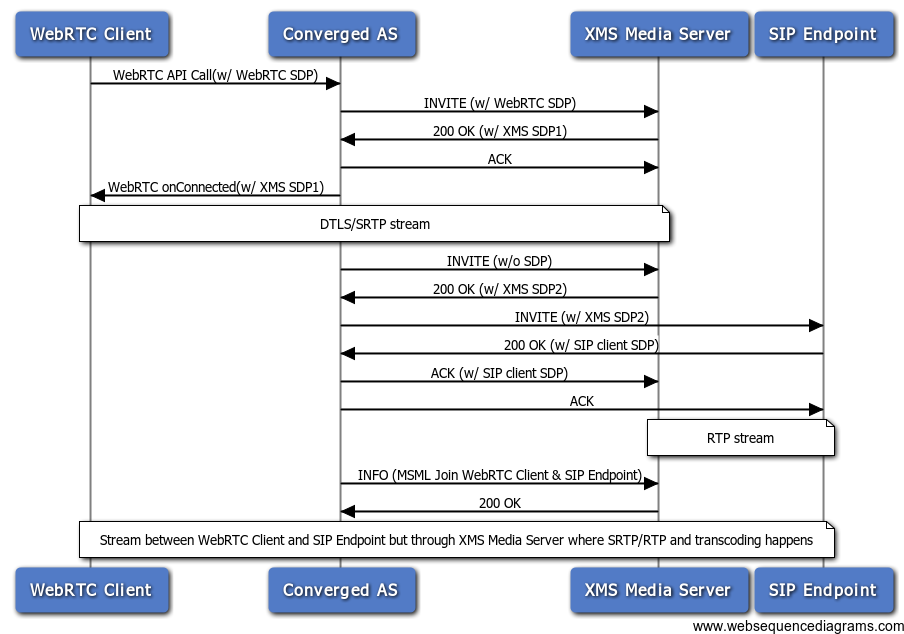
\includegraphics[width=0.95\textwidth,natwidth=610,natheight=642]{figs/chrome2xms.png}
  	\caption{Single Call from Browser to SIP Client}
  	\label{fig:chrome2xms}
\end{figure}

\par According to the documentation provided by Dialogic on XMS 2.1 \gls{rest}ful \gls{api}\cite{doc:xms_webapi}, it is only necessary to set \textit{encryption} field as \textit{dtls} and \textit{ice} as field \textit{yes} in the \gls{sdp} for \gls{webrtc} \gls{sdp} otherwise not set both fields for \gls{sip} \gls{sdp} when creating a call resource on XMS media server(shown at line 4 and 5 in Code Snippet \ref{code:xms}). It makes the interfaces on application server not necessarily be implemented differently for \gls{webrtc} and \gls{sip} clients.

\par In this sense, there are \textit{createXMSCall()}, \textit{joinXMSCall()}, \textit{updateLocalSDP()}, \textit{createConference()}, \textit{joinConference()}, \textit{deleteXMSCall()} and \textit{deleteXMSConference()} interfaces(shown in Code Snippet \ref{code:xms} ) implemented on application server by the reference of XMS 2.1 RESTful API User's Guide \cite{doc:xms_webapi}.

\par Using \textit{createXMSCall()} function as example of XMS integration implementation (from line 1 to line 37 in Code Snippet \ref{code:xms}), application server uses \textit{http} Node.js module and \textit{xml2js} Node.js module to implement this interface. Regards to XMS 2.1 \gls{rest}ful \gls{api}, creating call resource on XMS media server is a \textit{POST} \gls{http} request with configuration \gls{xml} as request content. From line 2 to line 7 n Code Snippet \ref{code:xms} is to generate the \gls{xml} content. And at line 8, application server calls \textit{http.request()} function with the \textit{option} object and callback function as arguments. The request \textit{option} object has \textit{host},\textit{port},\textit{method},\textit{path},\textit{headers} fields need to be set. The important point is that the \textit{Content-length} is necessary in the headers field, it is the length of the \gls{xml} content. These configuration is implemented from line 9 to line 17 in Code Snippet \ref{code:xms}. At line 35, application server calls \textit{req.write()} function to write \gls{xml} content data in \gls{http} request and sends it to XMS media server. There is a callback function along with the asynchronous function (\textit{http.request()}). In the callback function, application server needs to check the response data from the \gls{http} \textit{POST} request for useful \gls{sdp} data. By using \textit{xml2js} module object \textit{xmlparser} to parse the \gls{xml} data into \gls{json}, at line 26 and line 27, it is the process to strip the useful data \gls{sdp} from the response data. It is easier to keep using \gls{json} format for all the data object in Node.js as well as the application client. After the other process at line 28 and line 30, replacing some unsupported character in the \gls{sdp} for XMS media server by \textit{string.replace()} function, the \textit{createXMSCall()} function will return usful \gls{sdp} as result.

\begin{figure}
	\centering
    	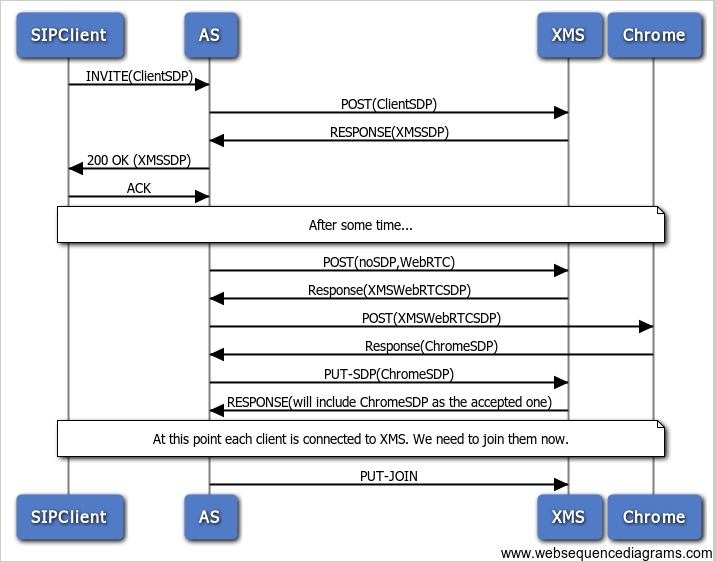
\includegraphics[width=0.95\textwidth,natwidth=610,natheight=642]{figs/sip2xms.png}
  	\caption{Single Call from SIP Client to Browser Client}
  	\label{fig:sip2xms}
\end{figure}

\par The rest of the interfaces for XMS media server on application server are similar with \textit{createXMSCall()} interface. \textit{joinXMSCall()} interface is made for single call resource join with another single call resource, it is used when a \gls{webrtc} call resource join a \gls{sip} call resource for single pair conversation in the prototype system. \textit{updateLocalSDP()} is made to update the \gls{sdp} of specific call resource on the XMS media server, but it does not work well against the current XMS media server when the \gls{webrtc} call resource is made without \gls{sdp} during the test and development. For this reason, the prototype application server can not use the normal process shown in Figure \ref{fig:sip2xms} when application server got a \gls{sip} \textit{INVITE} message. During the test, after creating the \gls{webrtc} call resource on XMS media server without \gls{sdp} and updating it later with the browser client answer \gls{sdp}, browser client fails to connect with the call resource on XMS media server in the \gls{rtp} session. To fix that, the application does the same process for the \gls{webrtc} part as the process shown in Figure \ref{fig:chrome2xms}. It means that no matter the \gls{webrtc} client is a receiver or a sender of the call request during the establishment, for \gls{webrtc} client itself will treat itself as a sender all the time, then the application server can always get the correct \gls{sdp} from the client to create the \gls{webrtc} call resource on XMS media server. This implementation of fixing solution is based on the WebSocket channels \textit{answer} and \textit{answerInvite} for both client side and server side Soket.IO code blocks with the \textit{self} flag value to see if the client is sender or receiver of the \textit{INVITE} message. This issue is reported to Dialogic team, hope it will be resolved in the future version of XMS media server.

\par \textit{createConference()} and \textit{joinConference()} are the corresponding interfaces against \textit{createXMSCall()} and \textit{joinXMSCall()}, they are made for conference resources usage on XMS media server. \textit{deleteXMSCall()} and \textit{deleteXMSConference()} are the delete functions for call resources and conference resources on XMS media server.

\section{Advanced Communication Function Implementation}

\noindent The most exciting reason for combining \gls{webrtc} technology with \gls{sip} \gls{voip} network is that there will be more advanced communication functions can be implemented under the power of web technology. There are two main advanced communication functions implemented in the prototype system.

\subsection{SMS Messaging}

\par \gls{sms} messaging is required for normal telephone usage. In the prototype system, it is necessary to have \gls{sms} messaging function during the conference if one of the participants is on his mobile phone only. The working prototype is shown in Figure \ref{fig:webgui_join_conference}. There are two peers in one conference, two of them are \gls{webrtc} clients(Gintel tester1, Gintel tester2) and one mobile phone client(Brian Chen). The implementation service is based on \gls{msg} provided by Gintel AS. It is a message service gateway for \gls{sip} clients to send \gls{sms} to other \gls{sip} clients or physical mobile phone. The implementation is shown in Code Snippet \ref{code:msg}. It uses the same \gls{http} Node.js module to implement the \gls{http} request communication with \gls{msg} server.

\begin{figure}
	\centering
    	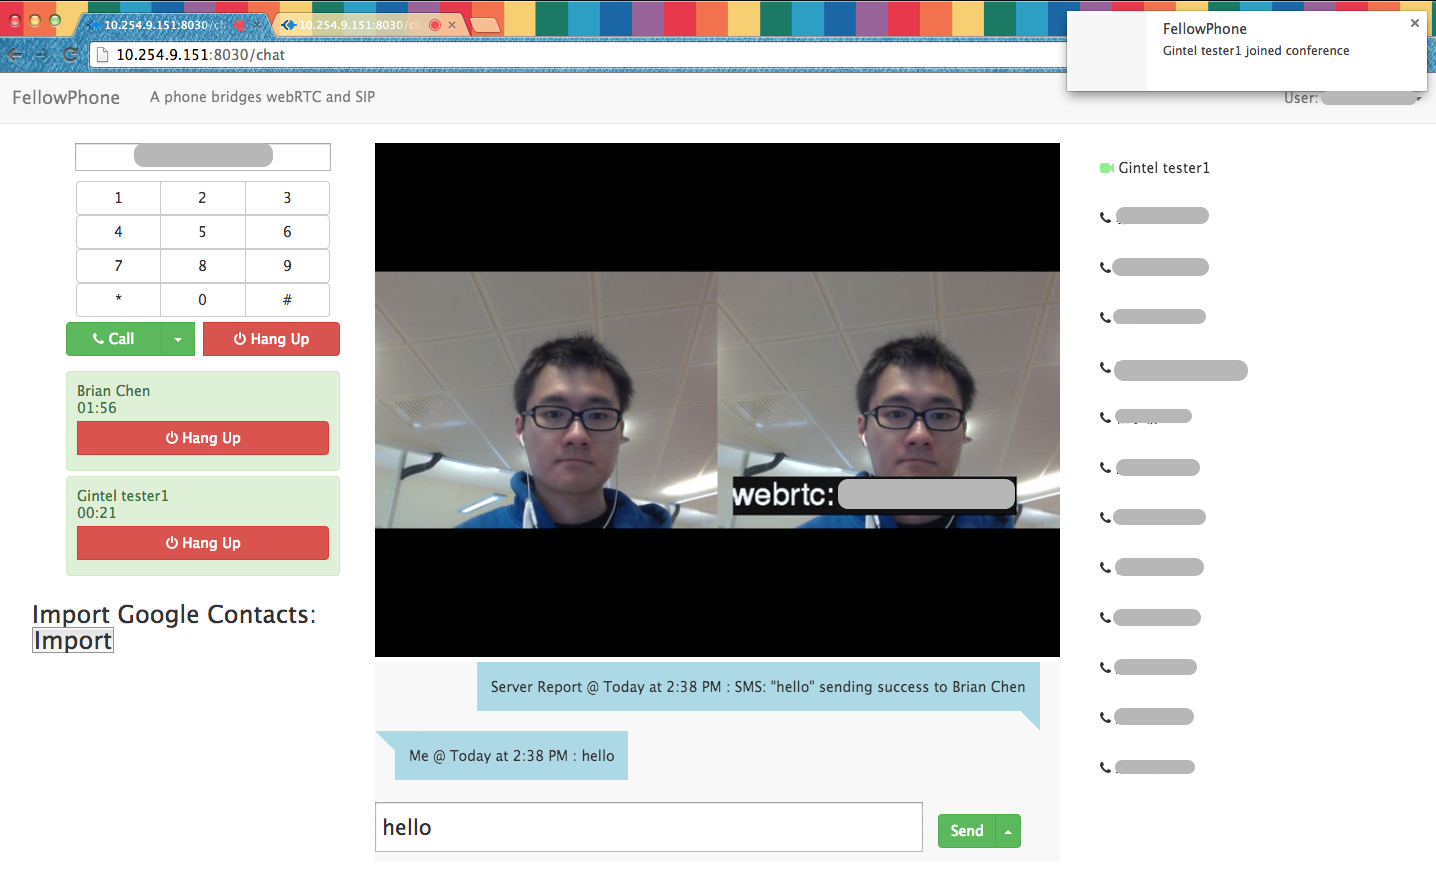
\includegraphics[width=0.95\textwidth,natwidth=610,natheight=642]{figs/webgui_join_conference.png}
  	\caption{Prototype Application in Conference Sending SMS}
  	\label{fig:webgui_join_conference}
\end{figure}

\par There are two steps to send \gls{sms} message. The first one is to get correct \gls{msg} user credential by providing the correct \textit{loginDto} object. \textit{loginDto} is a \gls{json} object generated with the user name and password. From line 2 to line 23 in Code Snippet \ref{code:msg} is the implementation of this process. It uses another Node.js framework library \textit{https.request()} function because of \gls{https} protocol is used on target \gls{msg}. This library can be used in the same pattern as \textit{http.request()} described before. However, \textit{https.request} takes only string text in the header fields, then at line 2 in Code Snippet \ref{code:msg}, it converts \gls{json} object into string. At line 13 in Code Snippet \ref{code:msg}, it is shown that if the credential sent to \gls{msg} server is correct, it will return a validate cookie in response data. This cookie will be used for second step to send \gls{sms} message. From line 25 to line 61 is the implementation of second step, the login credential and cookie need to be set in the header fields \textit{login} and \textit{Cookie}(shown at line 23 and 36). Moreover the message string is set in the \gls{http} request body at line 59, the \textit{Content-Type} and \textit{Content-Length} in the headers should be set as "application/json" and the length of message string content(it shows at line 33 and line 37).

\subsection{Files Sharing}

\par Because the \gls{rtp} media channel is connected with XMS media server for media  stream exchange, \gls{webrtc} \textit{RTCDataChannel} can not be used in this case. However, considering the prototype system is a real-time communication platform for collaboration working scenario, it is necessary for end points to have some collaboration tools such as files sharing. The screen shoot of file sharing in prototype application is shown in Figure \ref{fig:webgui_file_share_sender} and Figure \ref{fig:webgui_file_share_receiver}.

\begin{figure}
	\centering
    	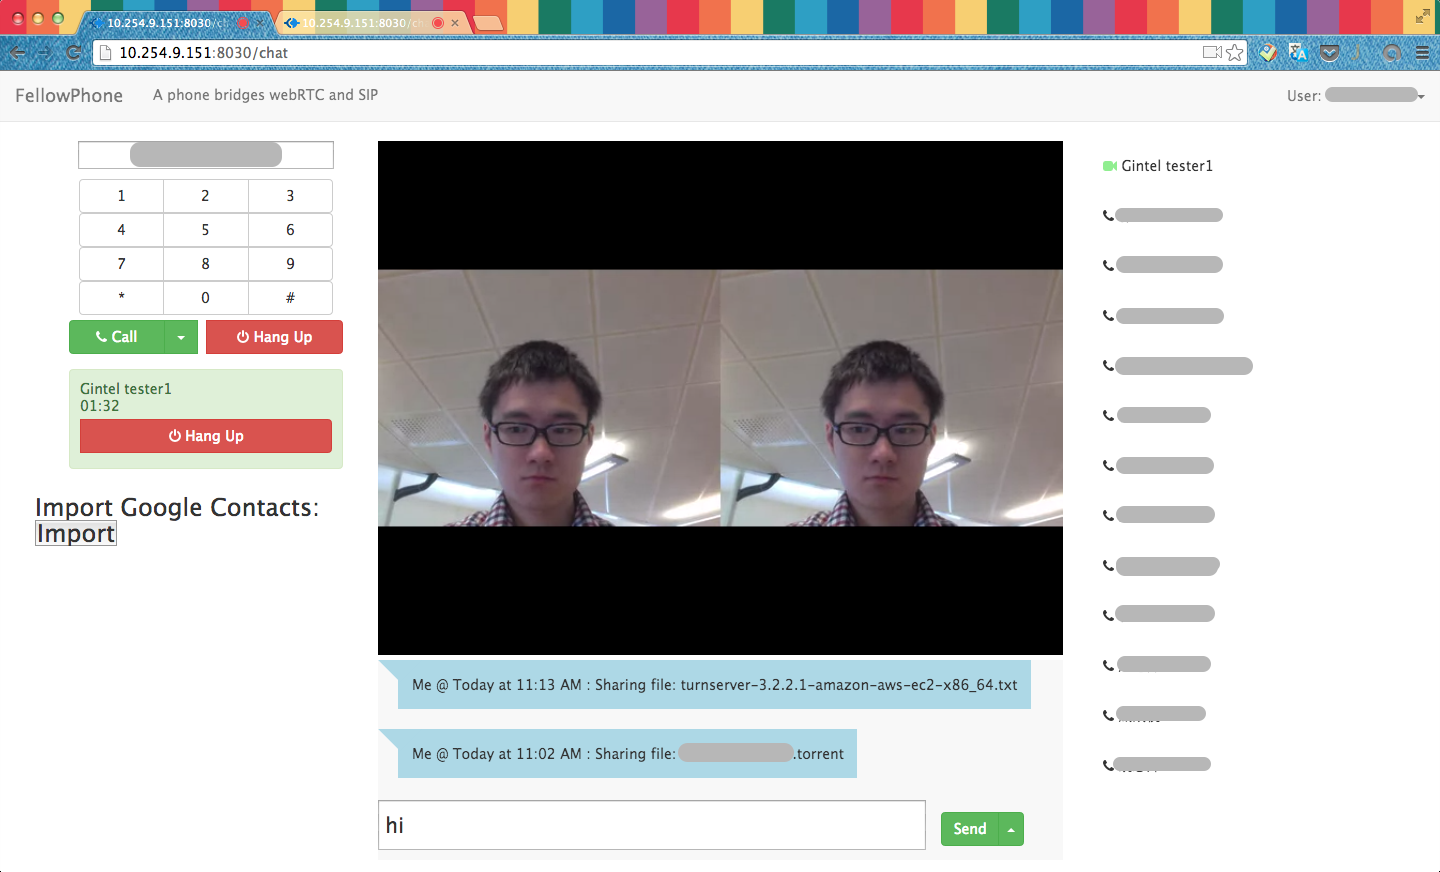
\includegraphics[width=0.85\textwidth,natwidth=610,natheight=642]{figs/webgui_file_share_sender.png}
  	\caption{File Sharing Sender Client}
  	\label{fig:webgui_file_share_sender}
  	    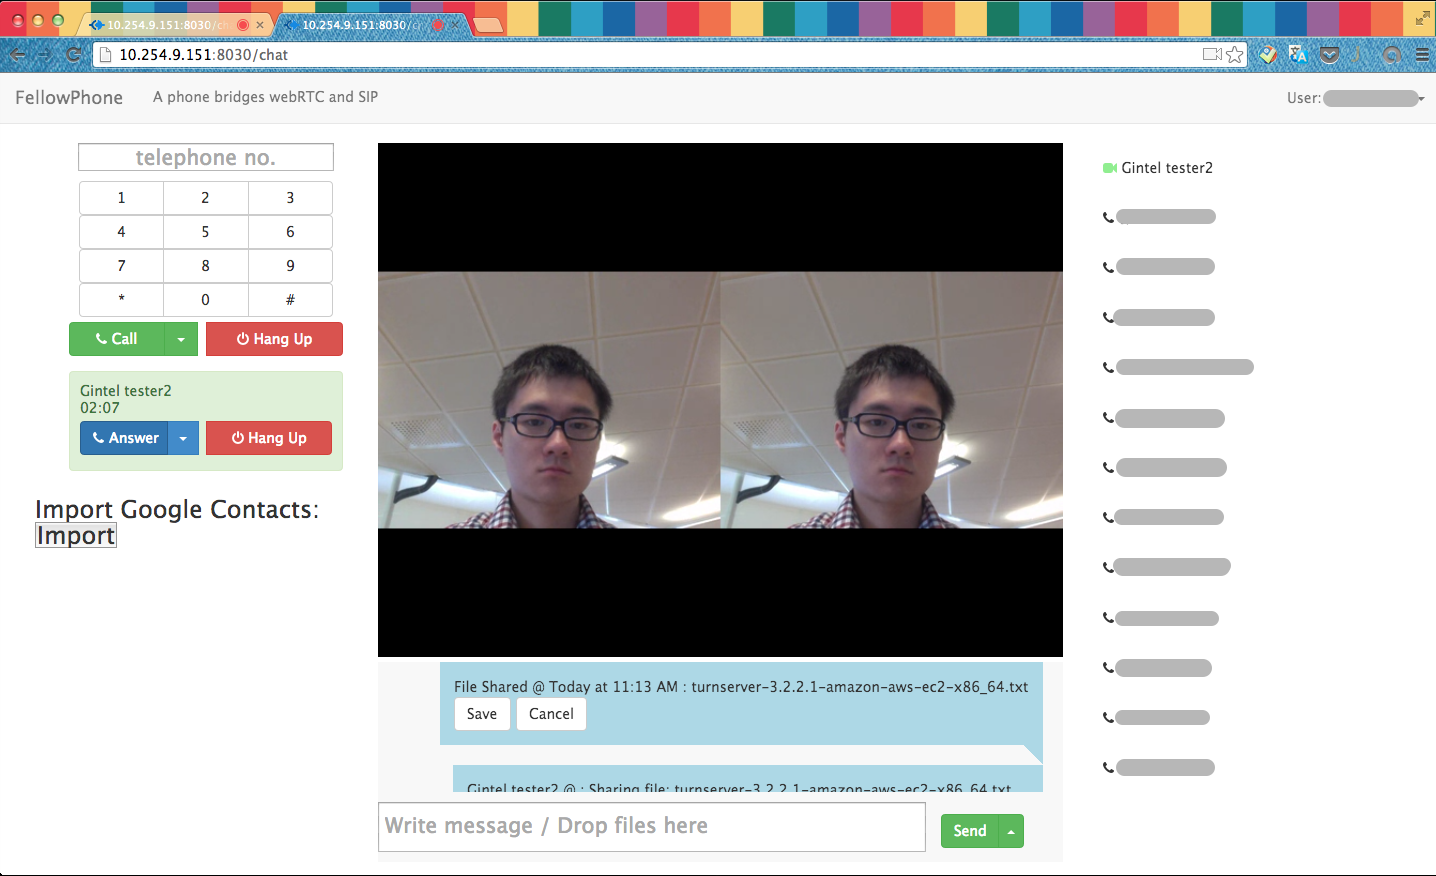
\includegraphics[width=0.85\textwidth,natwidth=610,natheight=642]{figs/webgui_file_share_receiver.png}
  	\caption{File Sharing Receiver Client}
  	\label{fig:webgui_file_share_receiver}
\end{figure}

\par As the screen shoot showing, when sender client uploads files to the application server, application server will directly share these files with the other clients in current conference session. The receiver client can decide whether these files need to be saved or not.

\par Prototype application uses Delivery.js library to do bidirectional File Transfers For Node.js via Socket.IO. Delivery.js uses Node.js and Socket.IO to make it easy to push files to the client, or send them to the server. Files can be pushed to the client as text (utf-8) or base64 (for images and binary files).\cite{github:deliveryjs} Since it is based on Socket.IO, it has the similar client and server implementation mechanism as Socket.IO. Once a WebSocket connection is established messages (frames) sent between the client and server contain only 2 additional bytes of overhead. In contrast, a traditional \textit{POST} request, and response, may have headers totaling 871 bytes. This could be a significant addition if many files are being sent, and would be even more significant if files are being divided into batches before being sent to the server. When pushing files to the client, the overhead of traditional polling methods provides an even starker contrast to WebSockets.

\par At line 9 in Code Snippet \ref{code:server_socket}, it declares the \textit{delivery} object using Delivery.js \gls{api} \textit{dl.listen()} with the Socket.IO \textit{socket} object as the argument. From line 36 to line 64 in Code Snippet \ref{code:server_socket} is the server side Delivery.js implementation code. It listens to the 'receive.success' WebSocket channel, when the upload files from client are received successfully the application server will make temporary files for the upload files and push these files to every connected clients in sender's current conference session. At line 38, application server uses \textit{fs.writeFile()} function from the Node.js framework \textit{fs} library to write the file byte data got from the client to the application server file system, then at line 46, it uses Delivery.js \textit{delivery.send()} function to push the file to the connected WebScoket client. For security reasons, the temporary files will be removed from the server when all the pushing process finished, it is implemented at line 54 by using \textit{fs.unlink()} function from Node.js framework \textit{fs} library.

\par After the files are pushed to the client, at line 42 in Code Snippet \ref{code:chatboard_ctrl}, the client side implementation will listen to the same WebSocket channel 'receive.success'. When there is file message from the application server to the client, the client listener will save the files in the runtime memory (it is not best solution for files sharing case, the improvement will be discussed in Chapter \ref{chp:future_work}), then let the user decide if these files need to be downloaded or removed. At line 32 in Code Snippet \ref{code:chatboard_ctrl}, it is the client side sending files function (\textit{delivery.send()}) to the server through WebSocket.

\begin{lstlisting}[caption={Files Sharing in ChatBoardCtrl.js},label={code:chatboard_ctrl}]
angular.module('webrtcDemo.controllers').
	controller('ChatBoardCtrl',function ($scope,$location,$upload,WebSocketService,storage,appId) {
		...
		function b64toBlob(b64Data, contentType, sliceSize) {
	    contentType = contentType || '';
	    sliceSize = sliceSize || 512;

	    var byteCharacters = atob(b64Data);
	    var byteArrays = [];

	    for (var offset = 0; offset < byteCharacters.length; offset += sliceSize) {
	        var slice = byteCharacters.slice(offset, offset + sliceSize);

	        var byteNumbers = new Array(slice.length);
	        for (var i = 0; i < slice.length; i++) {
	            byteNumbers[i] = slice.charCodeAt(i);
	        }

	        var byteArray = new Uint8Array(byteNumbers);

	        byteArrays.push(byteArray);
	    }

	    var blob = new Blob(byteArrays, {type: contentType});
	    return blob;
		}
        ...
		function _upload(files){
  		if(channelReday){
  			_.each(files,function(file){
  				...
					delivery.send(file);
  			});
  		}
  	}
  	...
		function _initChatBoardView(){
			socket = WebSocketService.getCurrentSocket();
			...
			delivery = new Delivery(socket);
			...
			delivery.on('receive.success',function(file){
	          $scope.recievedFiles.push(file);
	          ...	    
	      });
			...
		}
		...
  	$scope.saveFile = function(msg,filename){
  		var tempFile = _.find($scope.recievedFiles,function(file){
				return file.name == filename;
			});

  		var fileBlob = b64toBlob(tempFile.data,tempFile.mimeType);
  		saveAs(fileBlob, tempFile.name);
  		...
  	}
  	...
  });
\end{lstlisting}


\par Because Delivery.js sends files in base64\footnote{Base64 is a group of similar binary-to-text encoding schemes that represent binary data in an ASCII string format by translating it into a radix-64 representation. The term Base64 originates from a specific MIME content transfer encoding.\cite{wiki:base64}} encoding format, on the client application, it is necessary to convert base64 encoding string to Web \textit{Blob}\footnote{A Blob object represents a file-like object of immutable, raw data. Blobs represent data that isn't necessarily in a JavaScript-native format. The File interface is based on Blob, inheriting blob functionality and expanding it to support files on the user's system.\cite{mdn:blob}} data for using the \gls{html5} \gls{w3c} \textit{saveAs()} function to download file at line 55 in Code Snippet \ref{code:chatboard_ctrl}. The \textit{saveAs()} function takes Web \textit{Blob} object and file name as the two function parameters. The converting function is implemented at line 4 to line 26 as \textit{b64toBlob()} function in Code Snippet \ref{code:chatboard_ctrl}, it takes base64 string, content type of the file and slice size (in the prototype case it uses default 512 bit) to convert base64 string data to Web \textit{Blob} data. The important function in this code block is \textit{atob()}, it decodes a string of data which has been encoded using base-64 encoding, then slice the byte character data into byte array since \textit{Blob()} function only takes array of data objects, shown at line 24.

\par Based on these implementation for file sharing, it is even possible to send an E-mail with the sharing files as attachments to the current mobile phone(\gls{sip} client) participant in the conference on the application server. Although the mobile phone (\gls{sip} client) can not get the sharing files directly in real time, the user can still browser these shared files during the conference to discuss the topic with other participants.

